% !Mode:: "TeX:UTF-8"
\chapter{绪论}\label{chap:introduction}

\section{课题来源}

本课题来源于上海市公共卫生重点学科建设项目“基于新技术、新方法的放射卫生检测适宜技术研究”(编号:GWVI-11.1-40)。本文的研究受到上海市第六人民医院核医学科的数据支持和专家的技术支持并获得上海市第六人民医院伦理委员会的批准(编号:SH6H-2022-KY-113(K))。

\section{研究背景与意义}

骨骼是一种坚硬的器官\cite{morgan2021bone},构成了大多数脊椎动物骨骼的一部分。骨骼保护身体的其他器官,产生红细胞和白细胞,储存矿物质,为身体提供结构和支持,并使活动成为可能。骨骼有各种形状和大小,有复杂的内部和外部结构\cite{de2021vertebrate}。它们重量轻,但坚固耐用,具有多种功能。然而,骨骼系统也不免于面临各种疾病和损伤的威胁,其中感染性疾病是其中之一。

骨科相关感染是骨科手术和损伤后常见的并发症,涉及骨骼、关节、软组织等。主要包括骨髓炎、关节炎、滑膜炎、以及骨折相关感染和假体关节感染等。其中,骨折相关感染和假体关节感染是骨科手术中可怕且严峻的并发症\cite{sidiropoulos2022viral}。假体关节感染发生在人工关节(如人工髋关节、人工膝关节)的植入区域,对于新植入假体关节的患者来说有2\%-2.4\%的发病率,对于经历过翻修手术的患者可能达到20\%\cite{sconfienza2019diagnosis}。作为关节置换术后潜在的致命并发症之一\cite{niccoli2017bone,usuelli2019infections},假体关节感染可引起慢性疼痛、关节功能降低和其他导致患者身体不适的症状\cite{aleksyniene2022role}。假体关节感染常用的诊断方式有实验室检测、血清学、关节液抽取、微生物培养,但这些方法都没有完美的敏感性和特异性\cite{meermans2010there,parvizi2012mark,fink2013high,paul20142013,fink2018preoperative,claassen2014preoperative}。通常来说治疗方式包括手术清除感染组织、更换假体以及抗生素治疗。

另一方面,骨折相关感染曾称为创伤后骨髓炎,是骨损伤或创伤性手术后最严重的肌肉骨骼并发症之一\cite{govaert2020diagnosing},可能涉及手术创口感染、软组织受损引起的感染等,导致患病率增加、医疗费用昂贵和严重的诊断挑战\cite{metsemakers2017infection}。在骨折手术后,骨折相关感染的发病率为1\%-19\%\cite{ktistakis2014infection, malhotra2014open}。随着病情的发展,骨髓炎可伴有软组织感染,脓毒性关节炎伴或不伴皮肤窦道等一系列临床表现\cite{bhoil2019role},可能需要抗生素治疗、手术清创以及骨折修复等综合治疗手段。

虽然假体关节感染和骨折相关感染在发病原因和治疗方式上存在差异,但它们共同强调了在骨骼系统健康维护中的重要性。在美国初次全髋和全膝置换手术以及翻修手术的数量从2012年的52,134增加到2020年的2,224,587例。其中,全髋置换手术占总手术的52.1\%,全膝置换手术占34.6\%\cite{AJRR2021}。随着关节置换手术的数量逐年增加,美国每年大约有11,000个患者确诊假体关节感染\cite{kamath2015quantifying}。仅美国在2017年的假体关节感染治疗的估计成本就超过了10亿美元\cite{premkumar2021projected},而在美国骨折相关感染每年治疗的成本估计约为假体关节感染的四倍\cite{thakore2015surgical}。早期诊断、科学治疗和术后的有效康复是保障患者骨骼健康的关键,对于降低感染风险、减轻患者痛苦,降低医疗成本,以及维护骨骼功能都至关重要。

作为一种无侵入式的诊断方式,医学成像技术,例如超声、X射线、计算机断层成像(Computed Tomography, CT)、正电子发射断层显像(Positron Emission Tomography, PET)、单光子发射计算机断层成像术(Single-Photon Emission Computed Tomography,SPECT)、核共振成像(Magnetic Resonance Imaging, MRI)和骨三相(Three-Phase bone Scan, TBS)等等,可以提供人体内部结构和功能信息,被用于疾病的早期检测、诊断和治疗。其中,核医学成像技术通过注射放射性标记的物质,如放射性同位素,来追踪和测量骨髓、关节和周围软组织的代谢活动,从而提供更全面的信息。

\begin{figure}[ht]
  \centering
  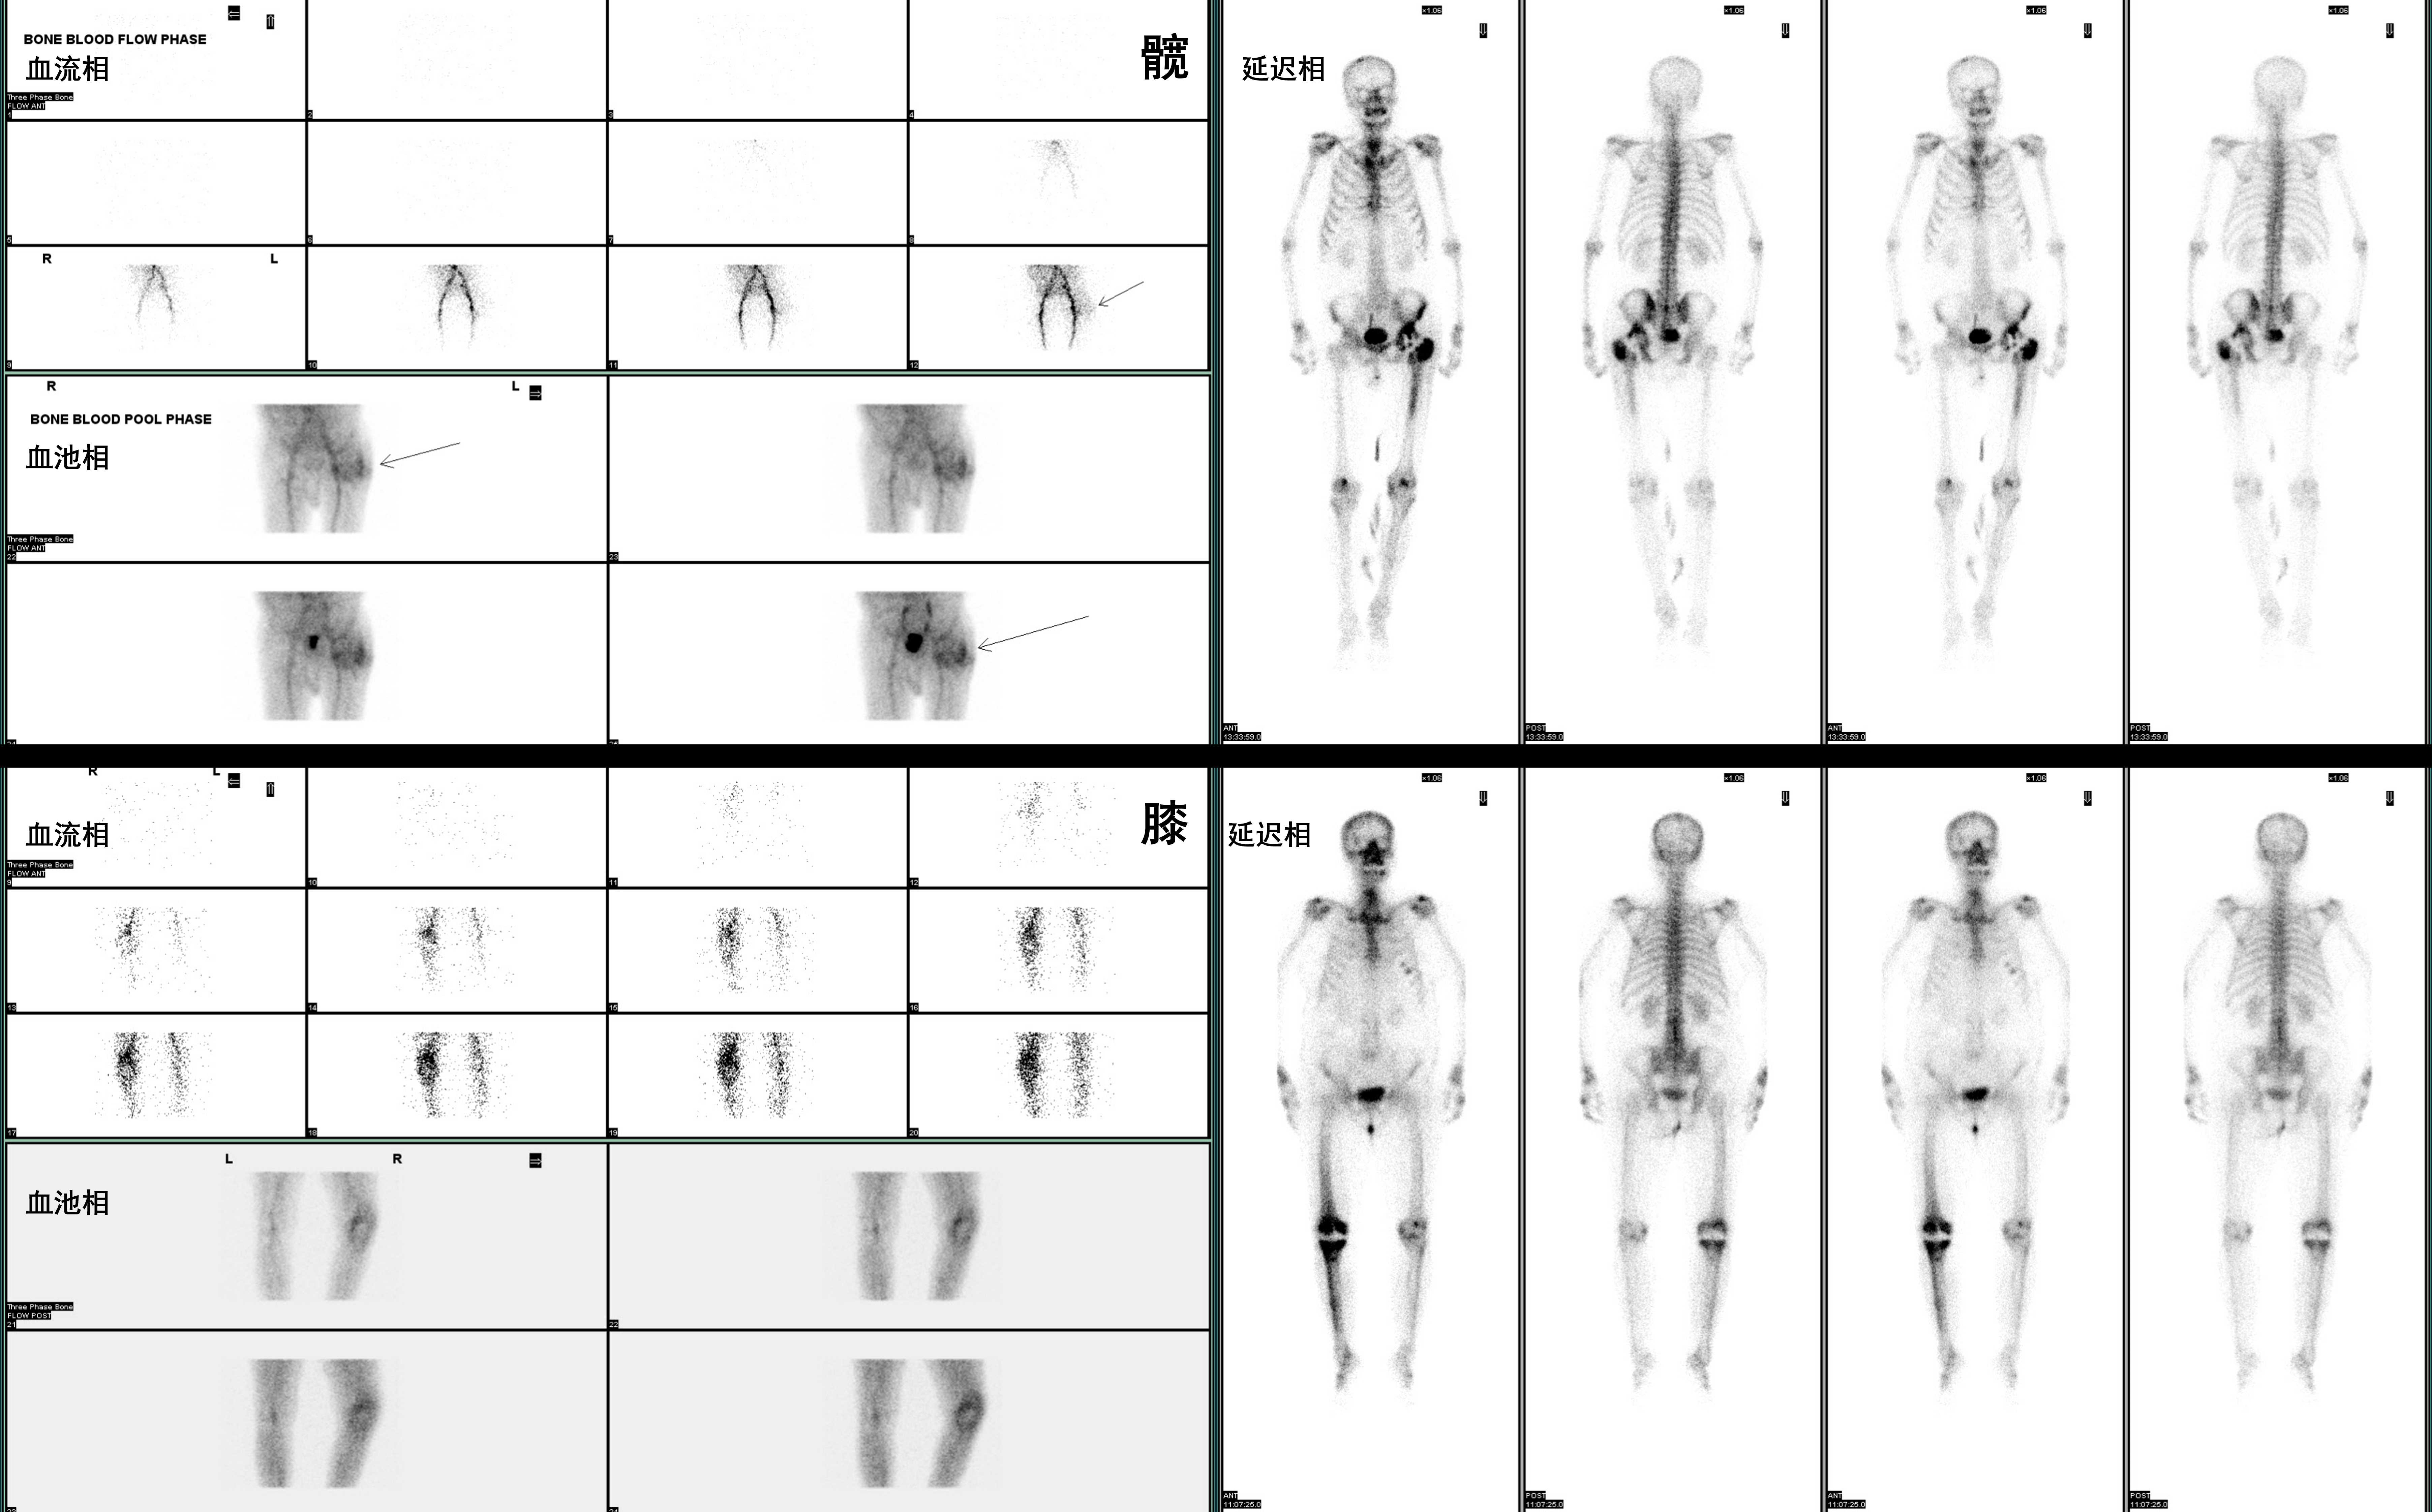
\includegraphics[width=\textwidth]{figures/chap01_DBS.png}
  \caption{\(^{99m}\)Tc-MDP 动态骨显像示意图}
  \label{fig:chap01_DBS}
\end{figure}

对于假体关节感染,核医学成像可以显示人工关节周围是否存在异常的代谢活动,揭示潜在的感染区域。如图\ref{fig:chap01_DBS},锝亚甲基二膦酸盐(\(^{99m}\)Tc-Methylene DiphosPhonate, \(^{99m}\)Tc-MDP)动态骨显像,也称之为骨三相,是核医学成像中第一个用于诊断假体关节感染的广泛可靠且简单影像模态\cite{niccoli2017bone}。Verberne等人\cite{verberne2016accuracy}的研究表明骨显像诊断全髋置换手术后的假体关节感染具有80\%的灵敏度和69\%的特异度。Kumar等人\cite{kumar2016comparative}发现动态骨显像在评估脓毒性的(或疼痛的)髋关节假体的敏感性、特异性和准确性分别为81\%、86\%和82\%。Zhang等人\cite{zhang2022temporal}通过在血流相中设定阈值的方法发现动态骨显像对膝关节假体感染的诊断灵敏度为94.3\%,特异度为56.0\%。根据文献和临床实践,动态骨显像诊断假体关节感染通常具有较高的敏感性,但特异性较低,尤其是经历过全膝置换手术的患者。

\begin{figure}[ht]
  \centering
  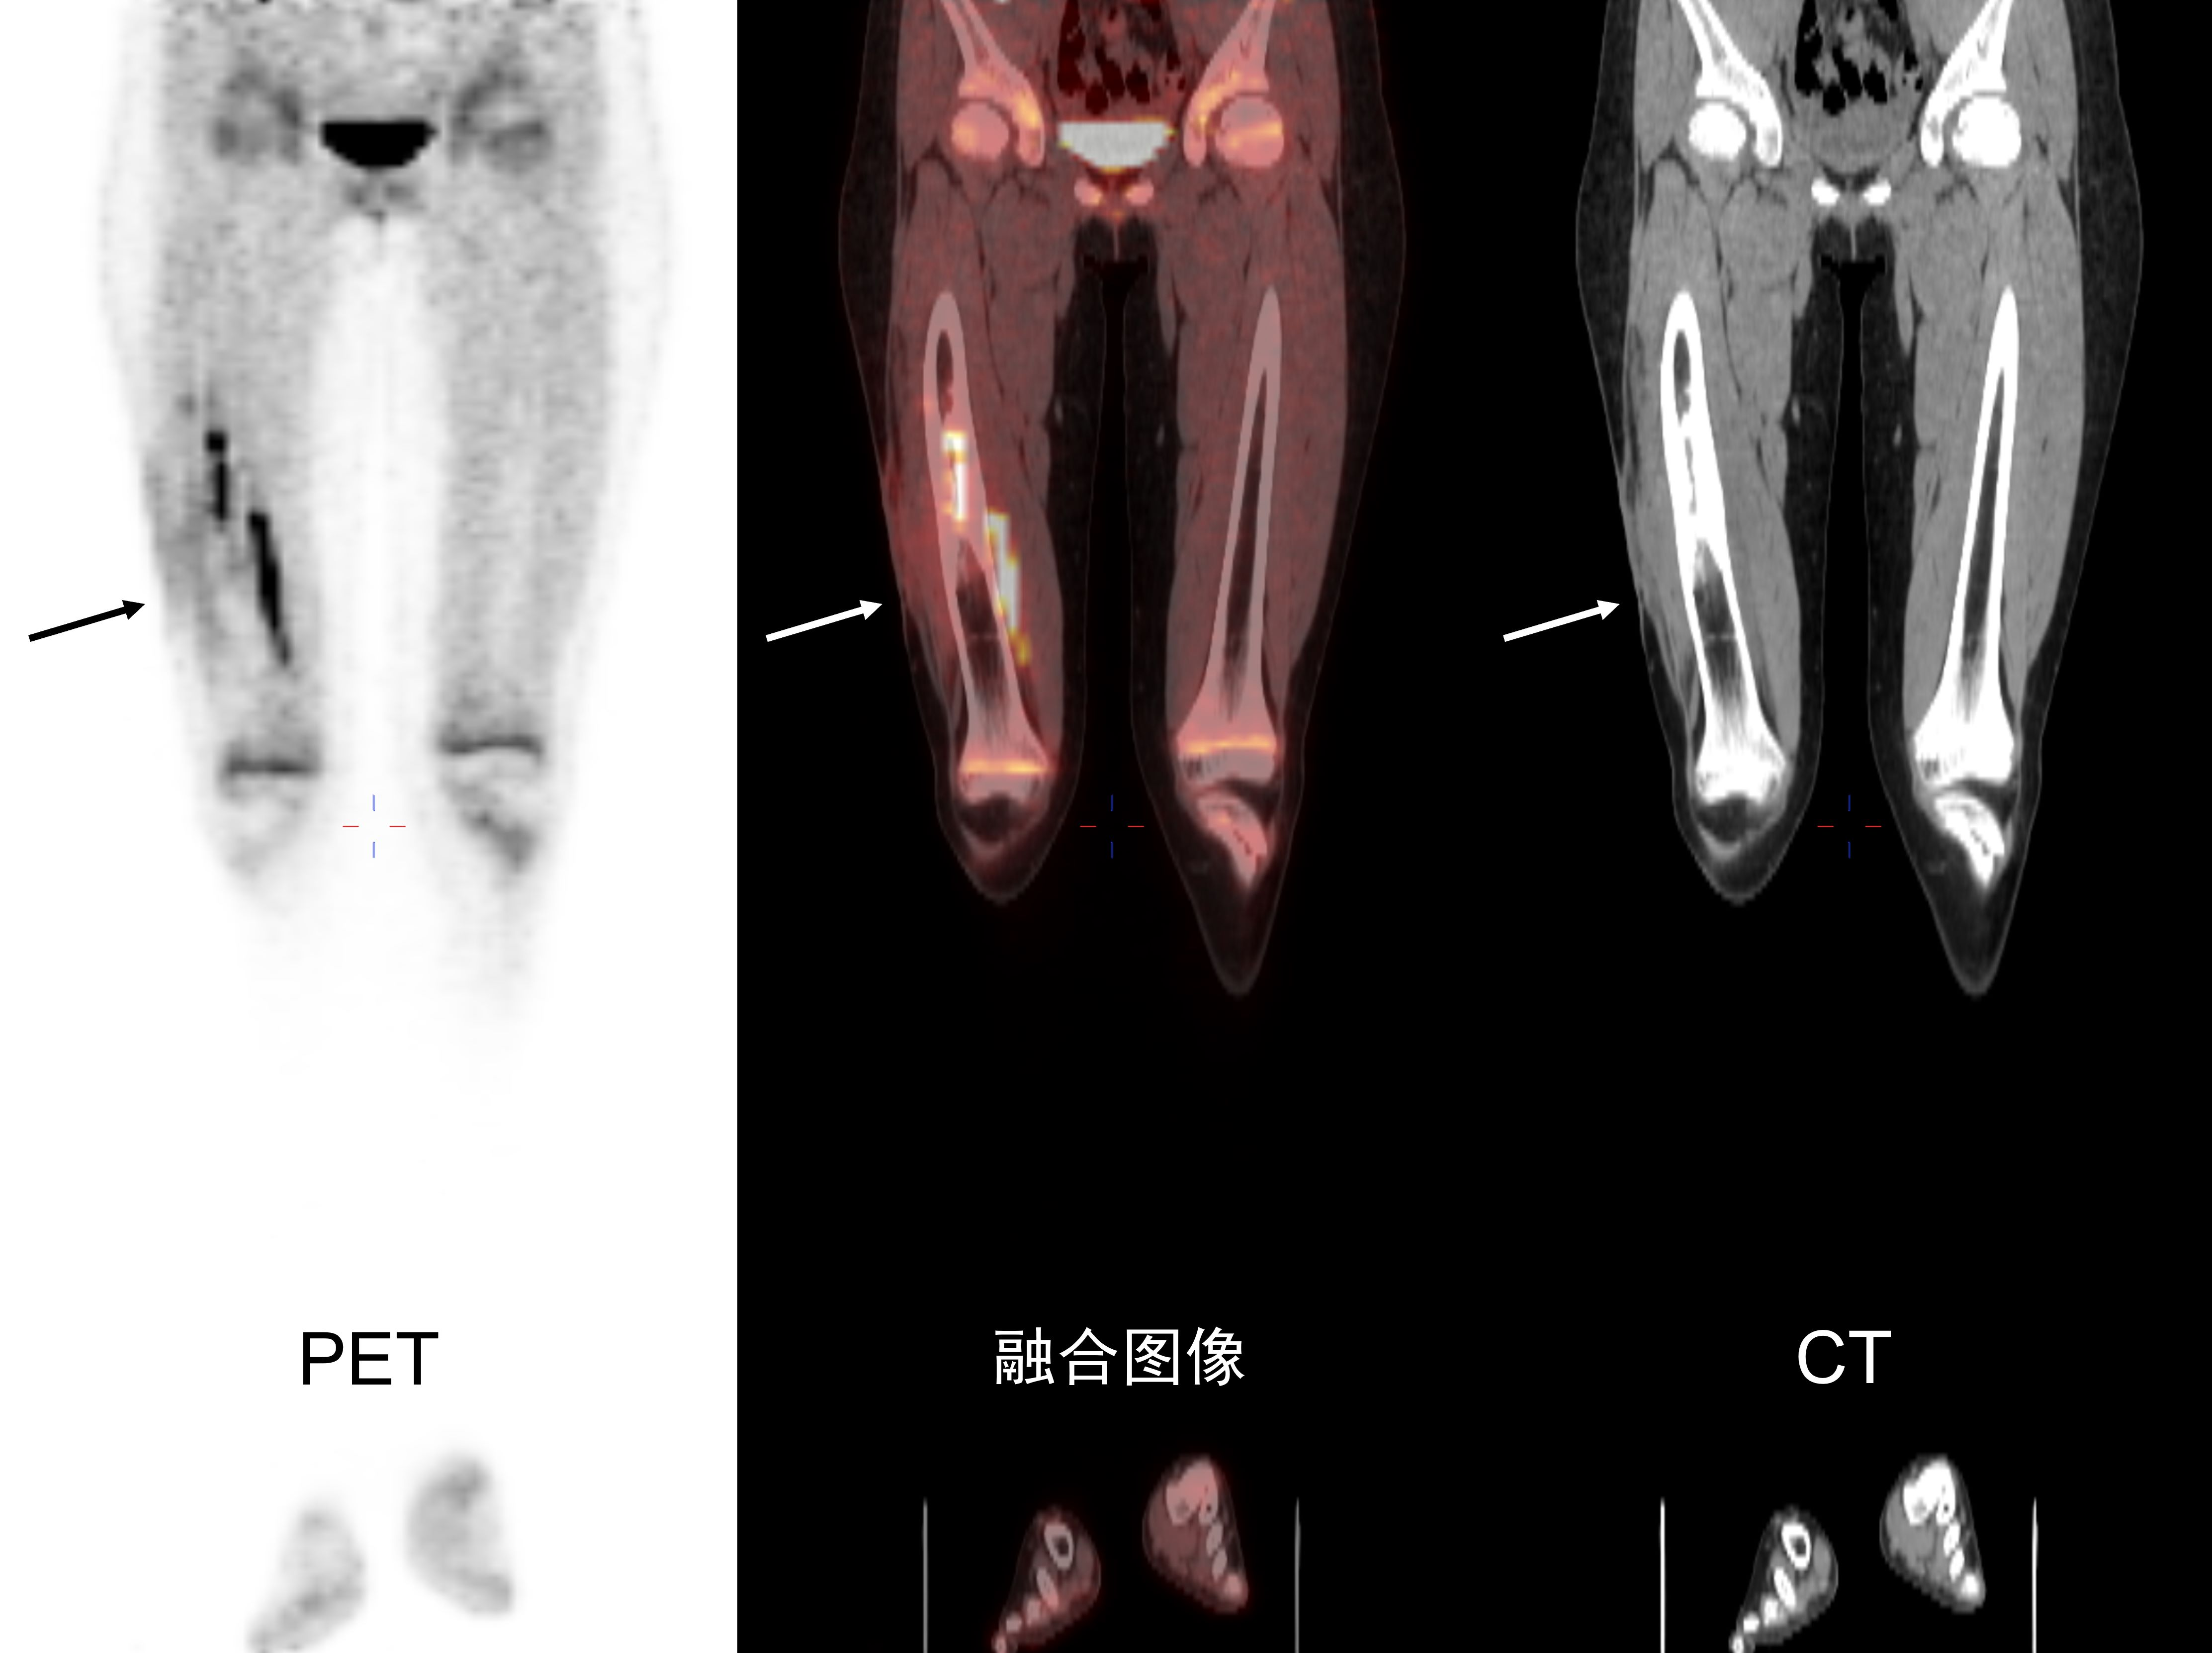
\includegraphics[width=0.8\textwidth]{figures/chap01_PETCT.png}
  \caption{\(^{18}\)F-FDG PET/CT示意图}
  \label{fig:chap01_PETCT}
\end{figure}

对于骨折相关感染,核医学成像则能够帮助定位骨折处是否存在感染迹象,有助于及早发现并采取适当的治疗措施。氟代脱氧葡萄糖(\(^{18}\)Fluorodeoxyglucose, \(^{18}\)F-FDG)PET/CT作为核医学的成像方式之一,常用于骨折相关感染的诊断\cite{zhang2021comparative},如图\ref{fig:chap01_PETCT}。它结合了解剖和生理信息,具有更高的空间分辨率和更好的量化可能性\cite{gholamrezanezhad2018clinical}。Lemans等人\cite{lemans2019diagnostic}通过在\(^{18}\)F-FDG PET/CT上量化分析,对骨折相关感染的准确率为83\%,阴性预测值为0.91。Wanter等人\cite{wenter2016diagnostic}研究发现,\(^{18}\)F-FDG PET/CT在慢性骨髓炎和骨科植入物相关感染中,阴性预测值为0.89、准确率为82\%。总体而言,\(^{18}\)F-FDG PET/CT在诊断骨折相关感染方面显示出令人满意的准确性。

近几年来,人工智能不断地发展,其在医学影像方面的应用也逐渐变成了关注的焦点。越来越多的深度学习方法被应用于医学影像领域的各种任务之中,如影像降噪,疾病分类,器官、组织和病灶的分割与检测、患者的预后效果预测等等\cite{ZSZD202307032,YJTY202304021}。以卷积神经网络(Convolutional Neural Network, CNN)、循环神经网络(Recurrent Neural Network,RNN)和基于注意力机制的Transformer为代表的深度学习方法因其优异的性能和较短的推理时间,经常被用来辅助核医学医生更迅速、准确地诊断病灶区域,减轻工作量。Liu等人\cite{liu2022diagnosis}(2022)提出了一种创新性多尺度CNN用于PET中阿尔茨海默病的诊断。Takahashi等人\cite{takahashi2022deep}(2022)提出了一个在PET/CT中对乳腺癌进行诊断的深度学习模型。然而,目前并没有用于假体关节感染和骨折相关感染这类骨科相关感染的自动化辅助诊断方法。为了有效地构建这种自动化辅助诊断方法,有几个问题必须前瞻性地加以考虑:

(1)数据集缺失。目前在网络上缺乏针对假体关节感染的动态骨显像数据集和针对骨折相关感染的PET/CT数据集。此外,医学影像数据集通常规模较小,来源相对单一,模型训练具有挑战性。

(2)髋关节的动态骨显像中存在生理上的高摄取区域,如膀胱和肾脏,这可能会使神经网络在进行分类时难以真正学习有用的信息并专注于病灶区域。其次,动态骨显像中包含血流相、血池相和延迟相(图\ref{fig:chap01_DBS}),且血流相和血池相中的图像序列具有时序性。因此,需要深入考虑如何充分利用动态骨显像的这些特点。最后,神经网络是一个缺乏解释的黑盒,这使得医生很难理解其预测的依据。

(3)尽管CT可以记录骨骼以及附近软组织的变化,但对骨折相关感染不太敏感。而PET中可以显示人体不同区域的代谢活性,且较高的标准摄取值反映了患有骨折相关感染的风险增加,但需要与炎症和愈合区分开来。其次,骨折相关感染的病灶区域仅占PET/CT整体影像的一小部分区域,且病灶的形状和位置多样,摄取的形式和程度也有所区别。因此,需要考虑到这些特征复杂性和多样性。最后,PET和CT都是三维的影像数据,这使得可以更全面地了解患者的解剖结构和生理活动。然而,这也给数据处理和模型设计带来了挑战。

(4)骨科相关感染的自动化辅助诊断方法应以简洁直观、易于操作的形式呈现,尤其对缺乏计算机和人工智能专业知识的用户尤为重要。首先,该方法需要整合骨科相关感染的自动诊断流程,具备智能分析的能力,以协助医生更快速地做出准确的诊断决策。其次,该方法需要提供图形化界面,以方便用户操作。最后,医学影像的可视化是必不可少的功能之一,并且提供一些辅助功能,满足大多数医学影像模态的需求,以便用户可直观地阅览影像。

由此,本文提出了四个主要的研究目标:

(1)构建数据集,收集真实患者的假体关节感染或骨折相关感染的影像数据和诊断报告,并进行数据清洗、标注和预处理工作。

(2)设计一个在动态骨显像上基于深度学习的假体关节感染辅助诊断框架,自动得出诊断结果,并通过类激活图等方法给医生提供决策依据和可信度。

(3)设计一个在三维PET/CT上基于深度学习的骨折相关感染检测与诊断框架,从PET/CT中自动定位出病灶区域并判断出病灶区域是否存在感染。

(4)设计一个骨科相关感染的自动诊断与可视化方法,不仅提供智能化功能辅助非专业人员进行假体关节感染和骨折相关感染的自动诊断功能,还能够满足用户简单直观地阅览与分析医学影像。

\section{研究内容与创新点}

\begin{figure}[htbp]
  \centering
  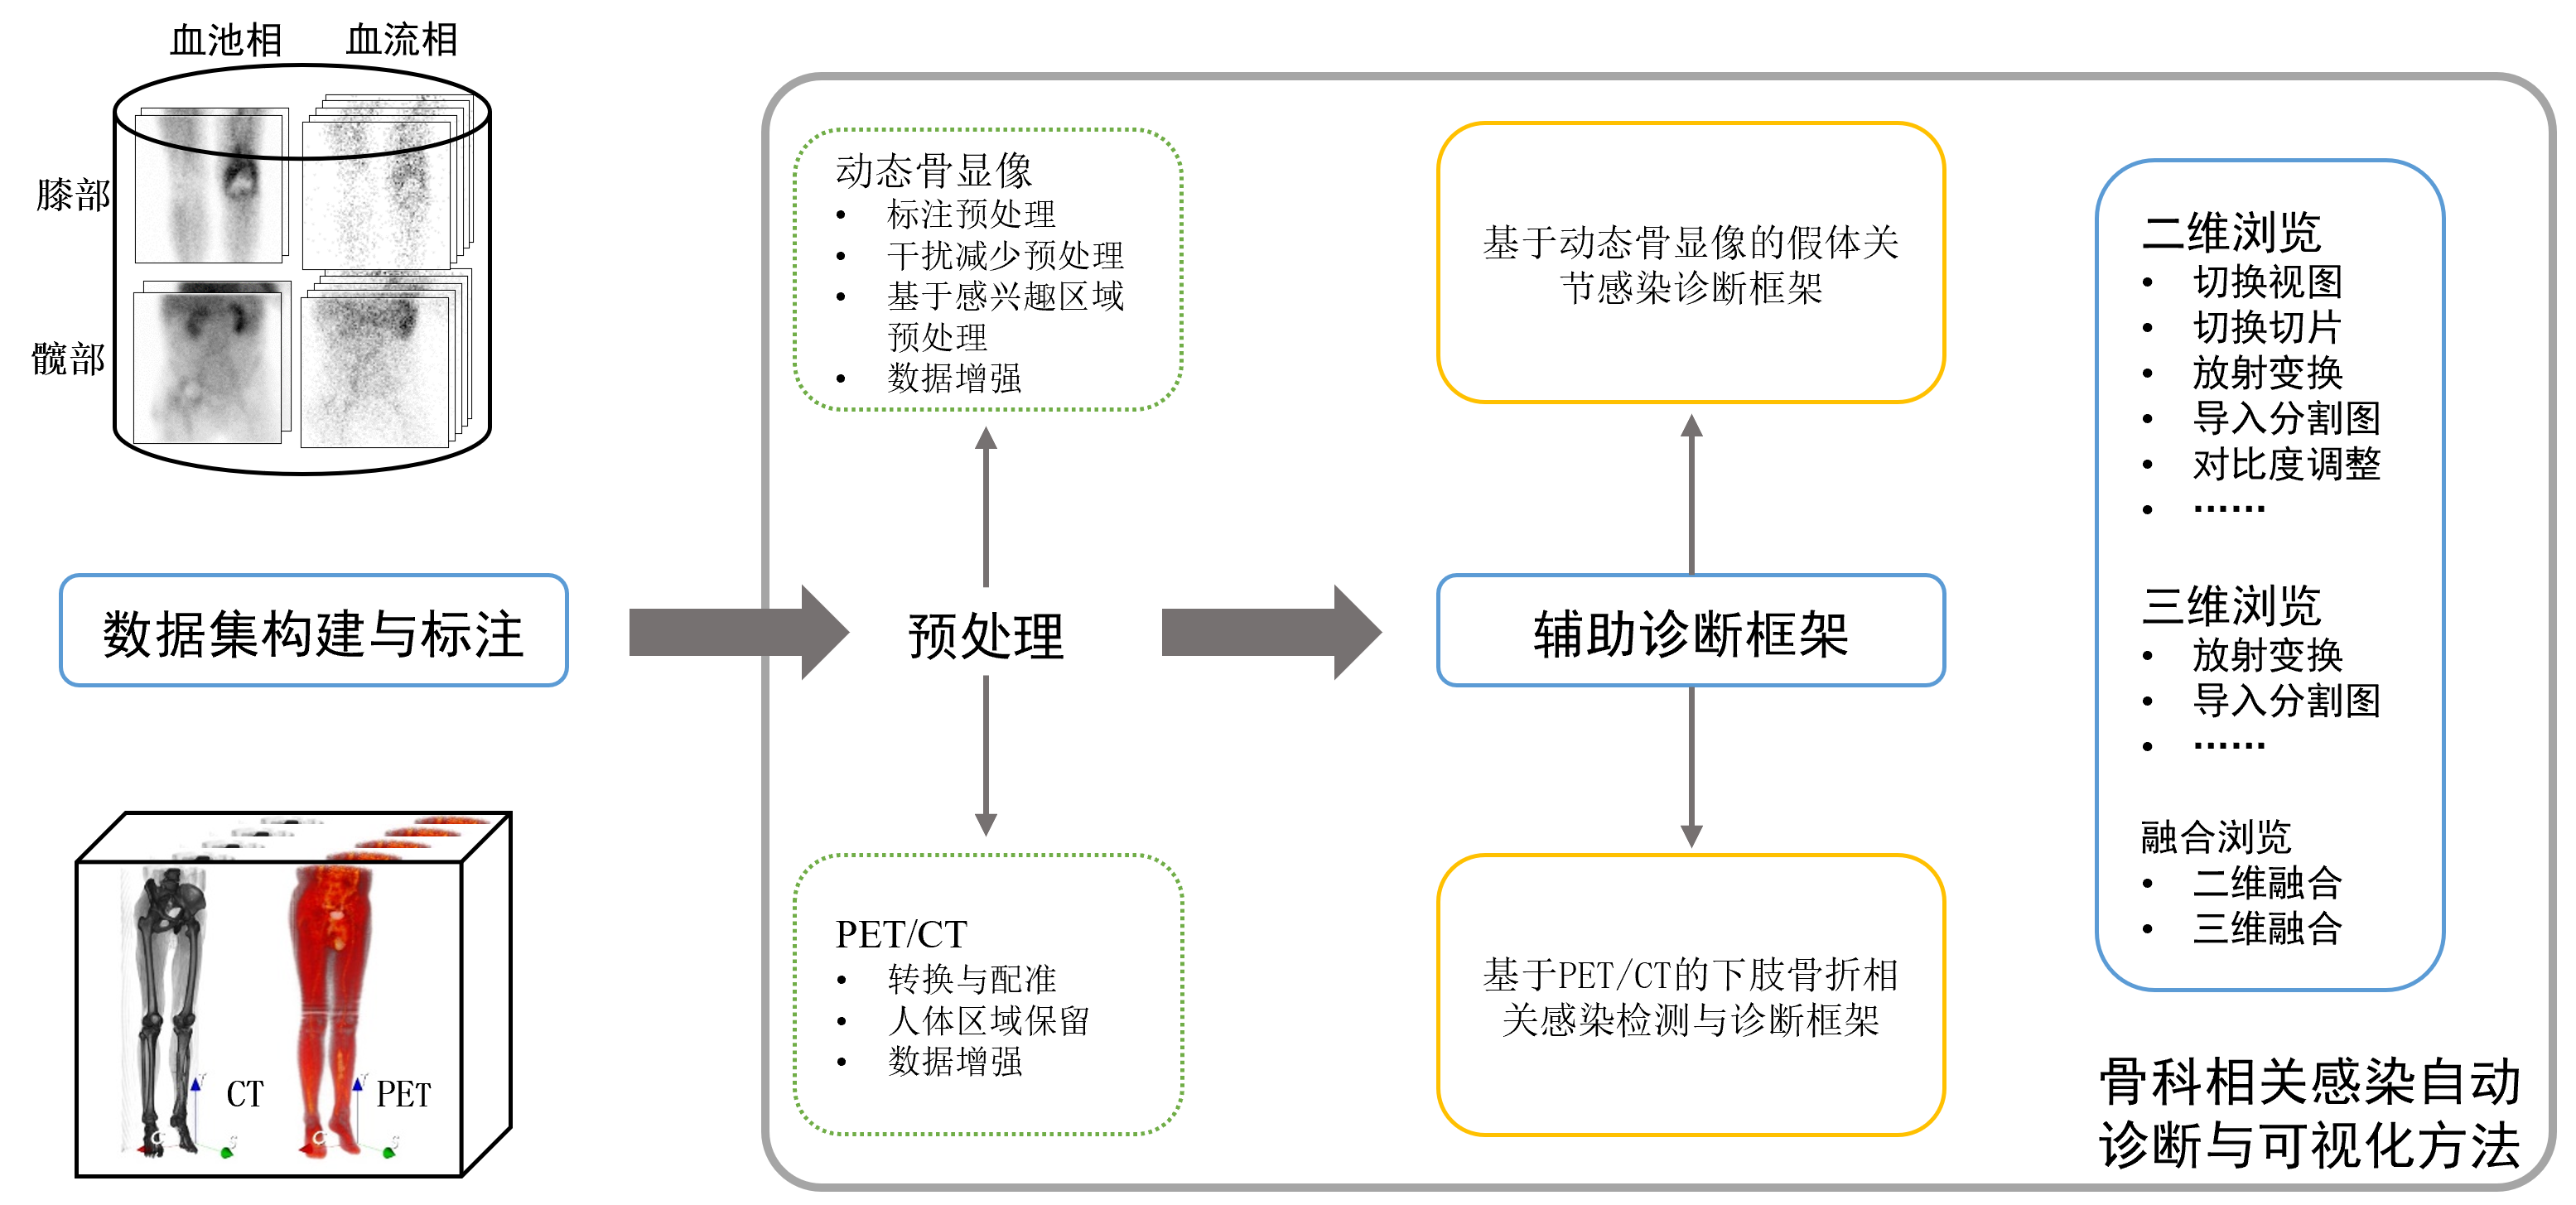
\includegraphics[width=\textwidth]{figures/chap01_research.png}
  \caption{本文的研究内容}
  \label{fig:chap01_research}
\end{figure}

根据1.2小节所述,本文围绕动态骨显像假体关节感染诊断分类任务、PET/CT骨折相关感染检测诊断任务以及骨科相关感染的自动诊断与可视化方法展开研究,主要研究内容和创新点如图\ref{fig:chap01_research}所示,包含以下四个部分:

(1)\textbf{数据集的构建与预处理方法的设计:}鉴于假体关节感染的动态骨显像数据集和骨折相关感染的PET/CT数据集的匮乏,本文作者与上海市第六人民医院核医学科合作,共同构建了两个重要的数据集。动态骨显像数据集纳入了在2016年1月至2021年6月期间455名患者的影像数据和相应的诊断报告,而PET/CT影像数据集则包含了2016年11月到2021年12月期间的281名患者的影像数据和诊断报告。在医学专家的指导下,通过仔细审查诊断报告和利用标注工具ITK-SNAP对数据集进行了详尽的标注工作,以确保数据的精准性和可靠性。针对动态骨显像和PET/CT影像,本文分别构建了高效的数据预处理方法。其中,动态骨显像采用了三种预处理算法和数据增强手段,而PET/CT影像则包括转换与配准、人体区域保留以及数据增强。这些预处理方法优化图像质量、标准化数据格式,并减缓无关区域和生理高摄取区域对模型性能的不良影响。

(2)\textbf{基于\(^{99m}\)Tc-MDP动态骨显像的假体关节感染辅助诊断框架:}为解决动态骨显像中假体关节感染诊断任务,构建了一种辅助诊断分类框架,由数据预处理和分类模型DBS-eNet组成。DBS-eNet结合了三维卷积和ConvLSTM,可以更有效地利用动态骨显像中不同相和相中的时序性图像序列。三维卷积用于在时序上提取不同相下每一张图像的生理摄取形态特征,ConvLSTM则捕捉和丰富单一图像的生理形态摄取特征,同时捕获图像序列中生理代谢的差异变化特征。实验结果表明,在五折交叉验证中,该框架在假体膝关节感染和假体髋关节感染的诊断任务上优于其他CNN,分类准确率分别达到了86.48\%和86.33\%;在独立验证中,该框架在假体膝关节感染上分类准确率达到了87.74\%,相比核医学专家们提升了13.55\%;在假体髋关节感染上分类准确率达到了86.36\%,与核医学专家们一致。统计学分析表明,该框架的诊断性能在假体膝关节感染上优于核医学专家,在假体髋关节上与核医学专家相当。

(3)\textbf{基于\(^{18}\)F-FDG PET/CT三维影像的下肢骨折相关感染检测与诊断框架:}为解决PET/CT影像中下肢骨折相关感染诊断任务,本文提出了一种全自动两阶段的检测与诊断框架3DFRINet。其中,3DFRINet 由病灶检测网络和病灶诊断分类网络构成。通过双分支设计和注意力模块,病灶检测网络能够捕获和融合不同模态的多尺度细节特征,从而精准地检测出病灶区域。病灶诊断分类网络通过最大强度投影将立体影像转换为平面图像,在获取有效特征的同时,对候选区域进行进一步挖掘,以捕捉骨折相关感染的代谢形态特征,从而实现对其准确的分类。实验结果表明,3DFRINet在下肢PET/CT影像中病灶检测性能优于其他YOLO模型,其AP\(_{25}\)达到了0.9234。在骨折相关感染病灶诊断分类任务中,该方法上达到了91.55\%的分类准确率和0.9250的F1,相比较于与初级核医学医生分别提升了11.27\%和0.1045,比高级核医学医生分别提升了4.32\%和0.0419。统计学分析表明,3DFRINet具有与初级核医学医生更好或相同的诊断能力,与高级核医学医生相当的诊断性能。

(4)\textbf{骨科相关感染的自动诊断与可视化方法:}为了构建一个假体关节感染和骨折相关感染的自动化辅助诊断方法,本文采用PyQt6框架,设计了一个骨科相关感染的自动诊断与可视化方法。该方法旨在为医生提供一款功能强大的辅助工具,具备全面而便捷的影像阅览和智能分析功能。在智能分析方面,该方法整合了(2)和(3)中的框架,以支持假体关节感染的诊断分类和骨折相关感染的病灶自动检测和分类。在影像阅览方面,该方法支持二维、三维和融合可视化,以满足不同医学影像模态的需求。二维可视化兼容大多数医学影像模态,提供显示视图、坐标和所在坐标值的信息,切换视图、几何变换等功能;三维可视化支持PET和CT,提供了旋转、缩放等功能;融合可视化支持PET和CT融合阅览,提供了二维和三维可视化功能。

\section{本文的整体结构}

本文基于作者攻读硕士学位期间的研究方向和参与的课题,分为六个章节,如图\ref{fig:chap01_structure}所示。各章节的内容安排如下:

\begin{figure}[htbp]
  \centering
  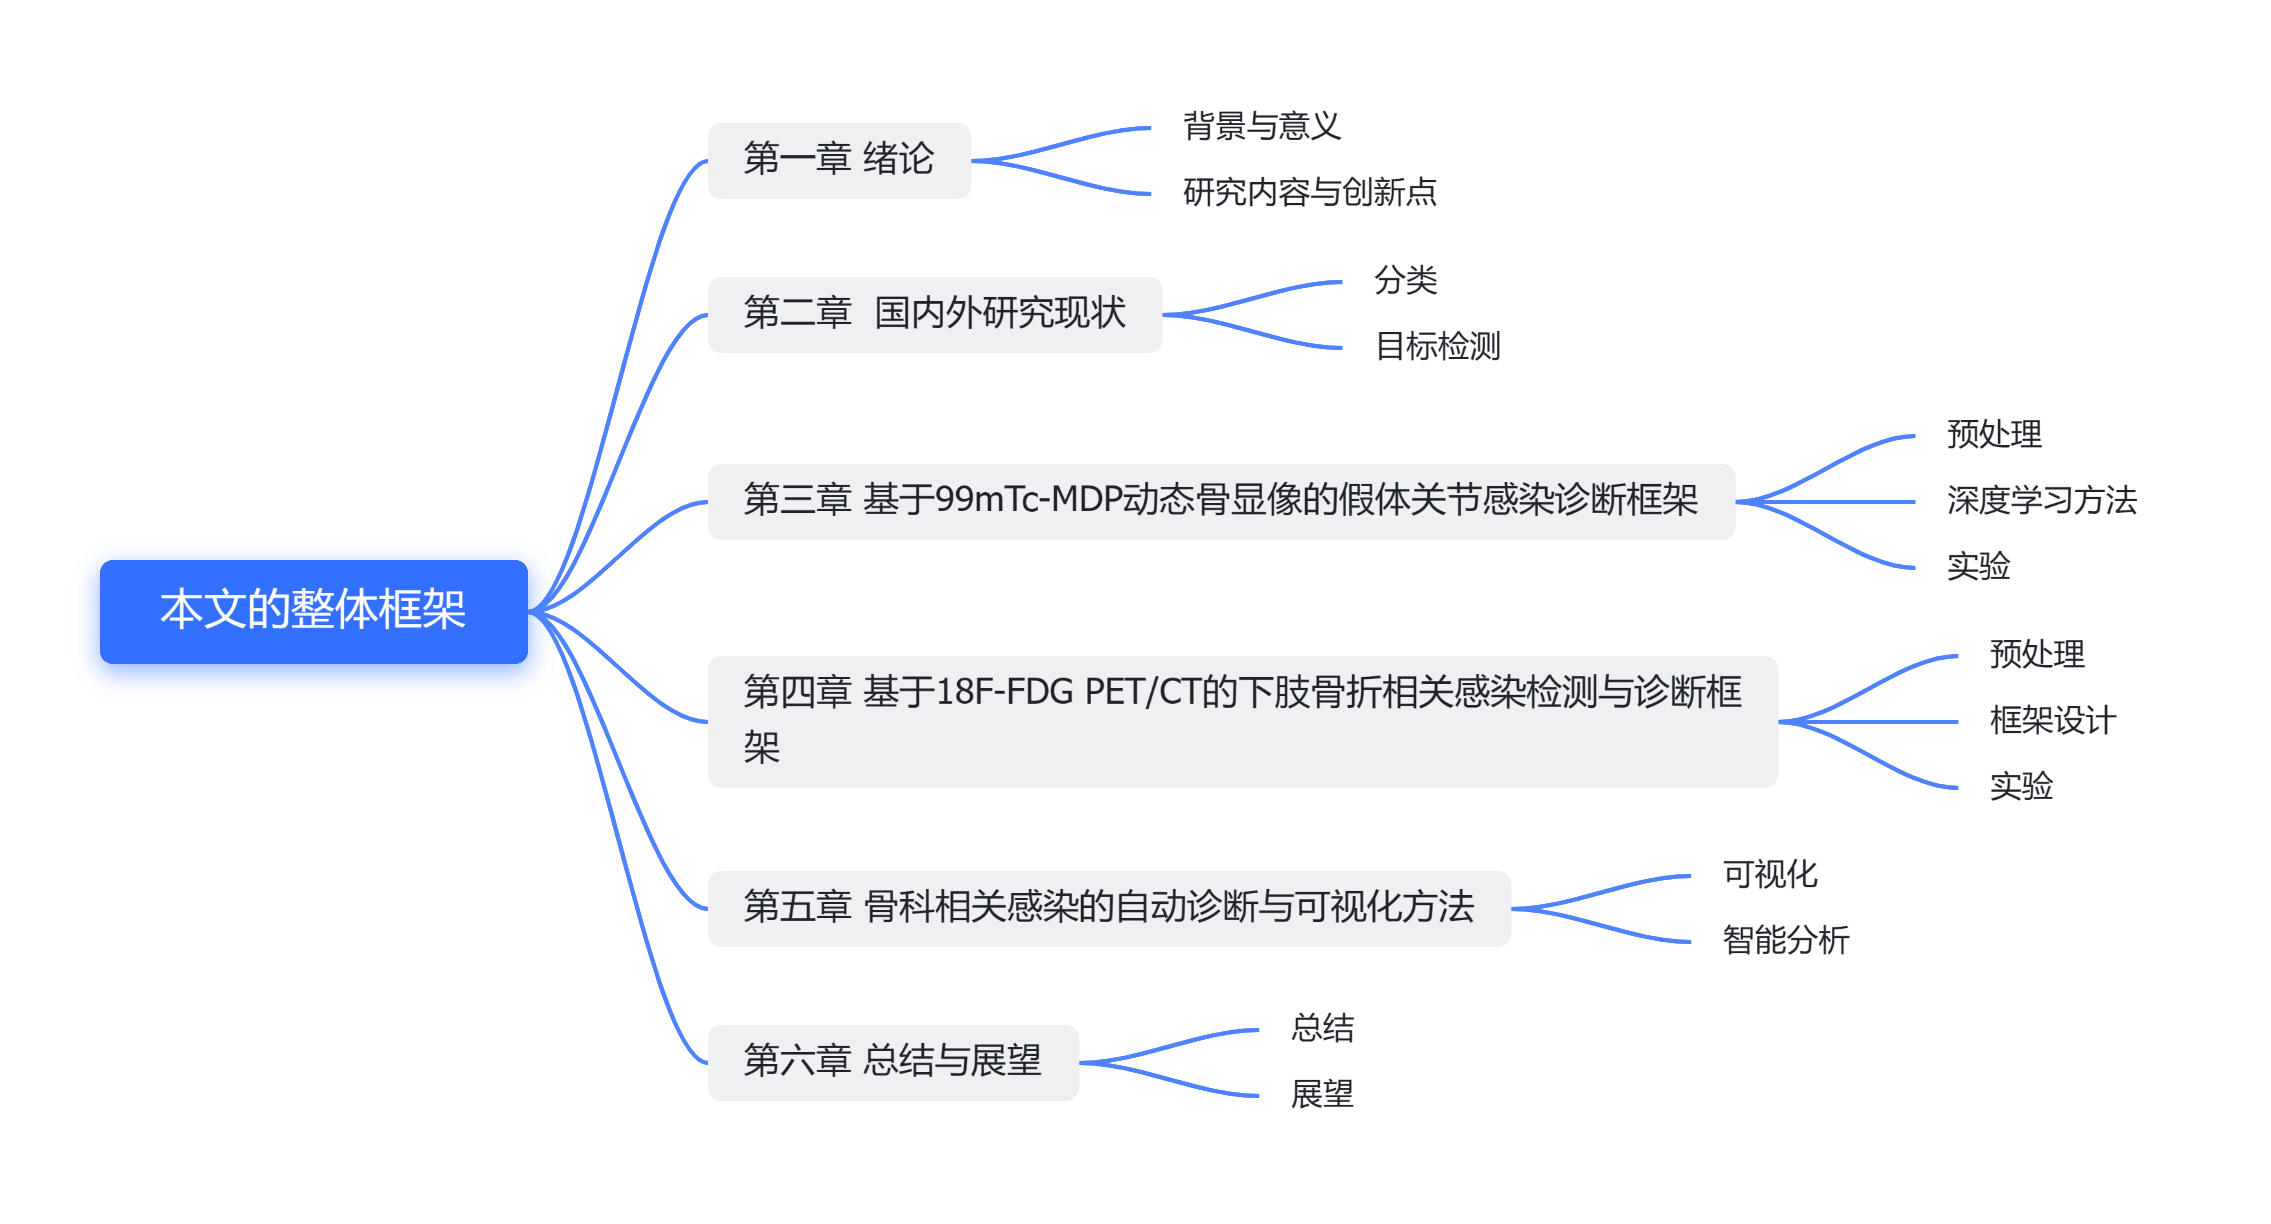
\includegraphics[width=\textwidth]{figures/chap01_structure_light.png}
  \caption{论文的整体结构}
  \label{fig:chap01_structure}
\end{figure}

第一章详细介绍了假体关节感染和骨折相关感染。接着阐述了深度学习方法与医学影像结合在骨科相关感染自动诊断方面的研究背景和研究意义,并介绍了研究的内容、目标和创新点。

第二章介绍了与本文研究内容相关的近几年国内外相关工作,总结了目前医学影像中分类和检测任务的研究进展,最后阐述了本文中假体关节感染和骨折相关感染诊断任务的特点,分析了任务的特殊性和现有的可行方法。

第三章从问题定义出发,详细介绍了基于\(^{99m}\)Tc-MDP动态骨显像的假体关节感染诊断框架。内容包括数据预处理方法、深度学习方法中模型的整体结构、损失函数以及用于展示模型可解释性的可视化方法。接着,通过一系列实验评估了该诊断框架的有效性和较好的诊断性能。

第四章同样从问题定义入手,详细介绍了基于\(^{18}\)F-FDG PET/CT三维影像的下肢骨折相关感染检测与诊断框架。内容包括数据预处理方法和框架设计。随后,通过一系列实验评估了该框架在病灶检测和诊断方面的出色表现。

第五章详细地介绍了骨科相关感染的自动诊断与可视化方法,拥有智能影像分析与影像阅览功能。

第六章对本文的研究工作进行了总结,并提出了未来可以进一步研究的方向。











